% Written by make_deck_figures.py: edit the script, not this file.
% The factor 1/max(|beta_i|, beta_floor)^xi_t on the expected growth rate, as in the left panel of Fig-L15a-BAB-Tilt.
\documentclass[tikz,border=2pt]{standalone}
% Shared style for the L15a schematics, copied from L14a (November 19, 2026), \input by each Fig-L15a-*.tex.
% Copied from week-13/L13a/figs/jumphmm-diagram.tex (the week-12 schematic style): same fonts,
% ink, accent colors, boxes, and arrows, plus a monospace font for tool names and order
% statuses. The notebook SVG carries a dark palette added by theme_svg.py; every color here
% must be mapped there.
\usepackage[no-math]{fontspec}
\IfFontExistsTF{Arial}{\setsansfont{Arial}}{\setsansfont{TeX Gyre Heros}}
\renewcommand{\familydefault}{\sfdefault}
\IfFontExistsTF{Menlo}{\setmonofont[Scale=0.92]{Menlo}}{}
\usepackage{amsmath,amssymb}
\usetikzlibrary{arrows.meta,calc,positioning,decorations.pathreplacing}

\definecolor{vnink}{HTML}{202124}
\definecolor{gdblue}{HTML}{0091FF}
\definecolor{gdred}{HTML}{E02020}
\definecolor{gdgray}{HTML}{6D7278}
\definecolor{saorange}{HTML}{F08C00}
\definecolor{boxfill}{HTML}{F1F3F4}
\definecolor{orangefill}{HTML}{FFE8C7}
\definecolor{bluefill}{HTML}{E5F3FF}
\definecolor{redfill}{HTML}{FDE8E8}
\definecolor{gridgray}{HTML}{E3E5E8}

\tikzset{
  every picture/.append style={x=1cm, y=1cm, font=\sffamily\small, text=vnink},
  % boxes and arrows, as in the L12a schematics
  flow/.style={draw=vnink, line width=0.9pt, -{Latex[length=2.4mm, width=1.7mm]}},
  feedback/.style={draw=saorange, line width=1.2pt, -{Latex[length=2.6mm, width=1.9mm]}, rounded corners=6pt},
  sumbox/.style={draw=vnink, fill=boxfill, line width=0.8pt, rounded corners=3pt, inner sep=5pt, align=center},
  note/.style={text=gdgray, font=\sffamily\footnotesize, align=center},
  state/.style={circle, draw=vnink, fill=white, line width=1.0pt, minimum size=1.1cm, inner sep=0pt, font=\sffamily\normalsize},
  % plots, as in the L10b profit diagrams
  axis/.style={draw=vnink, line width=0.8pt, -{Latex[length=2.6mm, width=1.8mm]}},
  spine/.style={draw=vnink, line width=0.8pt},
  curve/.style={draw=vnink, line width=1.6pt, line join=round, line cap=round},
  series/.style={draw=gdgray, line width=0.9pt, line join=round},
  drop/.style={draw=gdgray, line width=0.8pt, dash pattern=on 3pt off 2pt},
  pt/.style={circle, draw=vnink, fill=white, line width=1.0pt, inner sep=0pt, minimum size=2.0mm},
}


\begin{document}
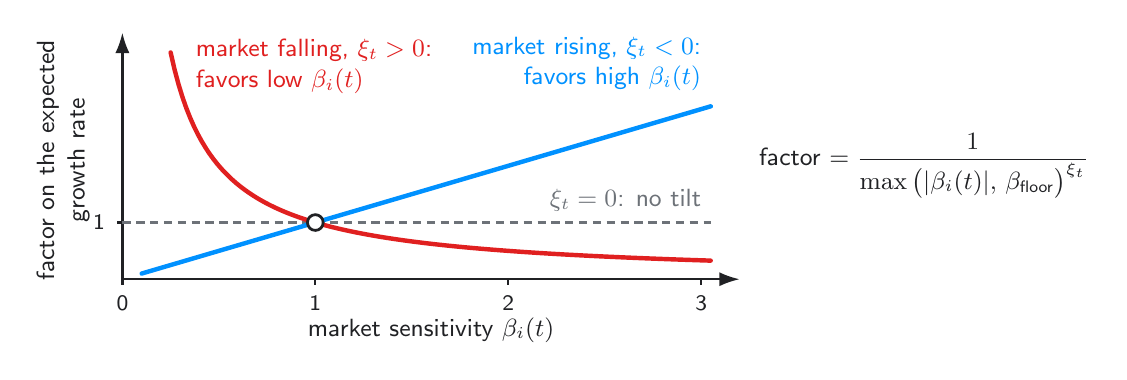
\begin{tikzpicture}
  \begin{scope}[x=2.45cm, y=0.72cm]
    \draw[axis] (0, 0) -- (3.2, 0);
    \draw[axis] (0, 0) -- (0, 4.35);
    \foreach \x in {0, 1, 2, 3} {
      \draw[spine] (\x, 0) -- (\x, -0.1);
      \node[anchor=north, font=\sffamily\footnotesize] at (\x, -0.12) {\x};
    }
    \draw[spine] (0, 1) -- (-0.03, 1);
    \node[anchor=east, font=\sffamily\footnotesize] at (-0.04, 1) {1};
    \node[font=\sffamily\small, anchor=north] at (1.6, -0.5) {market sensitivity $\beta_{i}(t)$};
    \node[font=\sffamily\small, rotate=90, anchor=south, align=center] at (-0.12, 2.1) {factor on the expected\\growth rate};
    \draw[drop] (0, 1) -- (3.05, 1);
    \draw[curve, draw=gdred] plot[domain=0.25:3.05, samples=140] (\x, {1/\x});
    \draw[curve, draw=gdblue] (0.1, 0.1) -- (3.05, 3.05);
    \node[pt] at (1, 1) {};
    \node[font=\sffamily\small, text=gdred, anchor=west, align=left] at (0.33, 3.75) {market falling, $\xi_{t}>0$:\\favors low $\beta_{i}(t)$};
    \node[font=\sffamily\small, text=gdblue, anchor=south east, align=right] at (3.05, 3.15) {market rising, $\xi_{t}<0$:\\favors high $\beta_{i}(t)$};
    \node[font=\sffamily\small, text=gdgray, anchor=south east] at (3.05, 1.02) {$\xi_{t}=0$: no tilt};
    \node[font=\sffamily\small, anchor=west] at (3.25, 2.0) {factor $=\dfrac{1}{\max\big(|\beta_{i}(t)|,\,\beta_{\text{floor}}\big)^{\xi_{t}}}$};
  \end{scope}
\end{tikzpicture}
\end{document}
